\documentclass[12pt,oneside]{article}
\usepackage{!sty/SBNart}
\usepackage{!sty/SBNsh}

%-------------------------------------------------------------------------------
% Info:
%-------------------------------------------------------------------------------
% *** Header:
\newcommand{\HdrL}{\normalfont \textsc{Technical Note} }%{ \normalfont \textsc{ELEC5508-2016S} }   
\newcommand{\HdrC}{}%{ \normalfont Course Outline}
%
% *** Title (\htitle)
\newcommand{\TopL}{Carleton Univ.~DoE}
\newcommand{\TopR}{Lecturer:~Dr.~Behzad~Nouri}
\newcommand{\midl}{ELEC5508~/~ELG6358\\ Computer Methods for Analysis and Design of VLSI Circuits}
\newcommand{\BotR}{Summer-2016}
%
%-------------------------------------------------------------------------------
\begin{document}
\isCUtitlefalse
\htitle{HSPICE\textsup{\textregistered} Primer}{Updated: \today}
%%-------------------------------------------------------------------------------
% Title W. Photo  -- Table of contents + colored
%-------------------------------------------------------------------------------


%-------------------------------------------------------------------------------
% Title + Photo:
%-------------------------------------------------------------------------------
\vspace{2cm}
{\color[rgb]{0,0,0.4}%{0,0.071,0.5}
\begin{singlespace}
\begin{center}
\mbox{\colorbox[rgb]{0.85,0.85,0.85}{%{0.85,0.85,0.85}{
\begin{minipage}[h]{0.85\textwidth} 
\HRule 
%--------------------------------------------------------
{\flushleft {\Huge \textbf{Teaching Dossier}}}\\
%--------------------------------------------------------
\HRule\\[3pt]
\begin{minipage}{0.4\textwidth}
\begin{flushleft} 
%--------------------------------------------------------
{\Large \textsc{\textbf{S.-Behzad Nouri}} }\\ \vspace{14pt}
{\large {Electronics Department} }\\ \vspace{6pt}
{\large {Carleton University} }\\\vspace{6pt}
{\textbf{email:}~~\href{mailto:bnouri@gmail.com}{\underline{bnouri@gmail.com}}}\\
%--------------------------------------------------------
\end{flushleft}
\end{minipage}
\begin{minipage}{0.4\textwidth}
\begin{flushright}
%\includegraphics[trim=0.5in 0in 0in 0in, scale=0.5]{sbn09}
%\includegraphics[trim=0.5in 0in 0in 0in, scale=0.2]{sbn11-1}
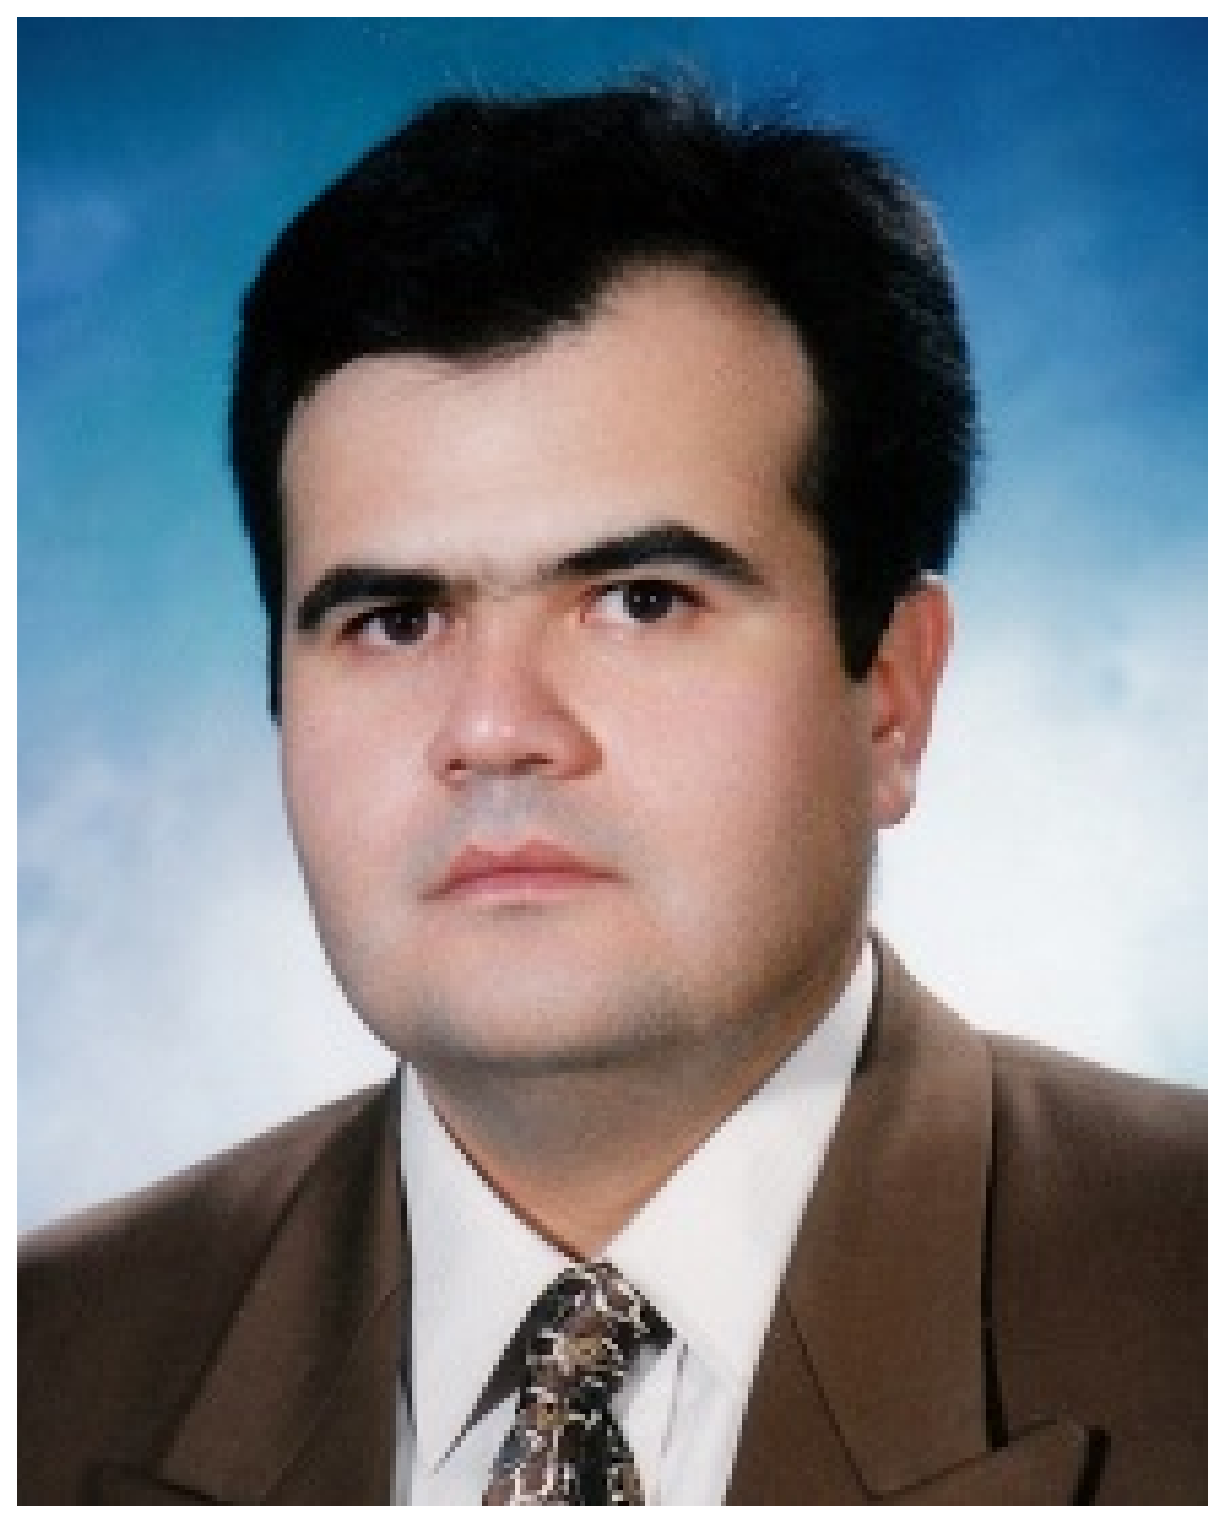
\includegraphics[trim=0.5in 0in 0in 0in, scale=0.12]{!opt/bn/sbn02c.eps}
\vspace{2pt}
\end{flushright}
\end{minipage}
\HRule 
\end{minipage} 
}} %\mbox
\end{center}
\end{singlespace}}



%-------------------------------------------------------------------------------
% Table of contents + colored
%-------------------------------------------------------------------------------
\begin{center}
%{\Large \textsc{\textbf{Cygwin~~Helps}} }\\ \vspace{14pt}  
\mbox{\colorbox[rgb]{0.92,0.92,0.92}{%{0.85,0.85,0.85}{
\begin{minipage}{0.75\textwidth}
\noindent \HRuleGray
\vspace{-12pt}
{\footnotesize \tableofcontents}
\noindent \HRuleGray
\end{minipage} }} %\mbox
\end{center}
\newpage

%---- End -------
\toc
%-------------------------------------------------------------------------------
% Title for Technical Note:
%-------------------------------------------------------------------------------
\rem{ % Simple Title for the Short Notes
	\mbox{}
	\begin{singlespace}
	\centering
	\textbf{\large Research Ideas}\\[6pt]
	\textbf{Behzad~Nouri}\\[4pt]
	Date:~August 23, 2016 %\today
	\end{singlespace}
} %rem
%-------------------------------------------------------------------------------

%-------------------------------------------------------------------------------
\section*{Entrance} \label{sec:entree}
%-------------------------------------------------------------------------------
This is a template!

%-------------------------------------------------------------------------------
\section{Introduction} \label{sec:intro}
%-------------------------------------------------------------------------------
Introduction goes here!
%
%-------------------------------------------------------------------------------
\section{Useful Command} \label{sec:useful}
%-------------------------------------------------------------------------------
This is as section with its own subsections including the fig.~\ref{fig:1} and \mbox{figures~\ref{fig:2}}-\ref{fig:3}
%-------------------------------------------------------------------------------
\subsection{Insert Figures} \label{sec:fig}
%-------------------------------------------------------------------------------
This is an example how a figure can be included in the \LaTeX file. The graphic formats including .png, *.jpg, *.pdf, and *.eps can be used.
\begin{figure}[!ht] 
\centering
\includegraphics[trim=0in 0in 0in 0in, , clip=true, keepaspectratio=true, width=31pc]{Figs/LinTL1.eps}
\caption{Linear transmission line circuit model.} 
\label{fig:1}
\end{figure} 
%
%
\par \noindent Also, figure can be inserted inline as \includegraphics[trim=0in 0in 0in 0in, , clip=true, keepaspectratio=true, scale=0.05]{Figs/cu1.png}, this time we use a figure of a ``*.png'' format.
%
%
\subsubsection{Figures side-by-side}
\begin{figure}[!ht]
\centering
\includegraphics[trim=0in 0in 0in 0in, , clip=true, keepaspectratio=true, width=31pc]{Figs/nouri-NLTL.eps}
\par{\small \textbf{(a)}}\par 
\mbox{ \begin{minipage}{0.5\textwidth}
\begin{flushright}
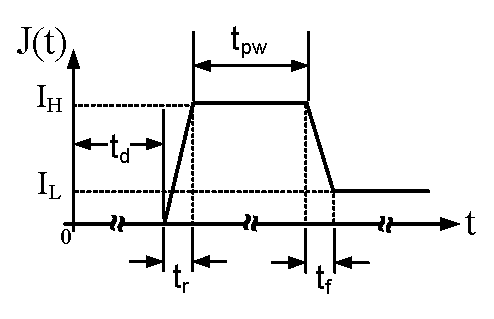
\includegraphics[trim=0in 0in 0in 0in, , clip=true, keepaspectratio=true, width=15pc]{Figs/nouri-NLTL-Jt.eps} 
%\vfill
\end{flushright}
\end{minipage}
\hspace{-8pt}
\begin{minipage}{10pc}
\begin{flushleft}
\begin{align*}
\mathrm{I_H}    &= 10, &\mathrm{I_L}  &= 1   \\
\mathrm{t_d}    &= 2,  &\mathrm{t_r}  &= 0.5  \\
\mathrm{t_{pw}} &= 15, &\mathrm{t_f}  &= 0.5  \\
\end{align*}
\end{flushleft}
%\vspace{30pt}
\end{minipage} }
\par{\small \textbf{(b)}} 
\caption{(a)~Nonlinear transmission line circuit model; (b)~Excitation waveform at input.} 
\label{fig:2}
\end{figure} 
%
%
\begin{figure}[!ht]
\centering
\includegraphics[trim=0in 0in 0in 0in, clip=true, keepaspectratio=true, width=21pc]{Figs/EX2_Iin.eps}  
\\{\small \textbf{(a)}} \\
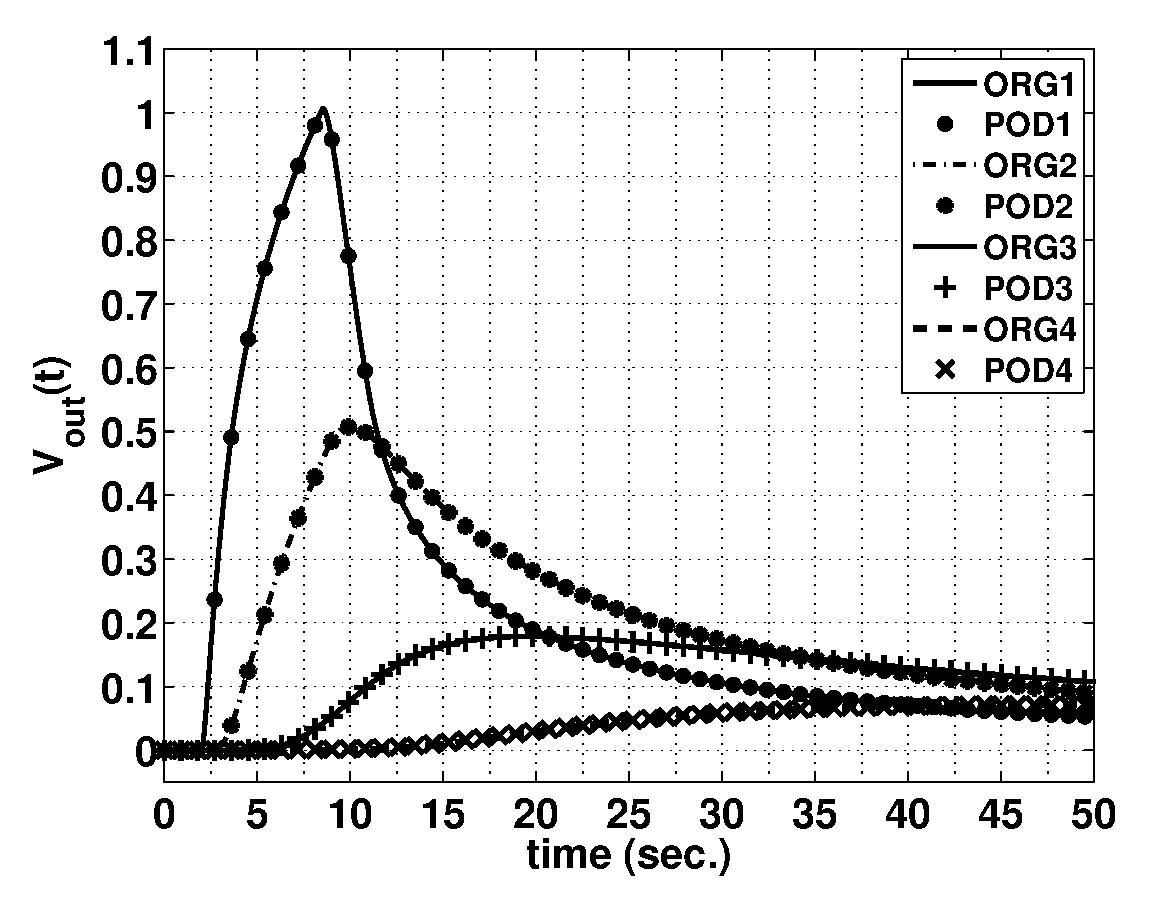
\includegraphics[trim=0in 0in 0in 0in, clip=true, keepaspectratio=true, width=21pc]{Figs/EX2_resp.eps} 
\\{\small \textbf{(b)}} \\
\caption{(a)~Excitation test waveform at input; (b)~Comparison of the responses at nodes 5, 50, 70, and 200, respectively.}
\label{fig:3}
\end{figure} %
%
\newpage
\subsubsection{Equations in \LaTeX}
%
Let include an inline equation $x=2$ or a bigger equation in the file. We will refer to it as \eqref{eq:2}.
%
%
\begin{equation}
\label{eq:1}
\mat{A}=\left[
\begin{array}{ccc}
 1 &-2 & 3 \\
-4 & 5 & 6 \\
 7 & 8 &-9
\end{array} 
\right]
\end{equation}
%
%
One may want to do some fancy stuff (e.g.) as shown in \eqref{eq:2}.
%
%
\begin{equation}
\label{eq:2}
\mat{A}=\left[
\begin{array}{c|c|c}
 1 &-2 & 3 \\
\hline
-4 & 5 & 6 \\
\hline
 7 & 8 &-9
\end{array} 
\right]
\end{equation}
%
%
If an equation is too big to be written in one line We also can split it in two or more lines as shown in \eqref{fig:3}.
%
%
\begin{multline}
\label{eq:3}
x=q+w+E+r+t+y+u+i+O+p+a+S+D+F+G+H+j+k+l= \\
SSSSS+L_{11}\times lllll\times (zxc*vbn)^3/2
\end{multline}
%
%
May be there are formulas or equations that may look better if the are written in two lines or more as 
%
%
\begin{align}
\label{eq:4}
x &= A+b+C \nonumber  \\
  &= \pm Y^{10}_{ex}  \\
	&= z
\end{align}
%
%
The following is sample of a bit twisted way of including an equation.
\begin{equation} \label{eq:10}
\begin{array}{*{20}{c}}
\begin{array}{l}
\textnormal{Error\;in}\\
\textnormal{Trajectories}\;\mlii{\buildrel \Delta \over =}
\end{array}
\sqrt{\dfrac{\sum\limits_{j = 1}^N \; \sum\limits_{i = 1}^n {\left( {x_i^{(org)}(j)-x_i^{(mor)}(j)} \right)}^2}{n \times N}}
\end{array}
\end{equation}
%
%
Next, in the \mbox{appendix~\ref{app:fancy}}, you will find more facy stuff that you may want to take advantage from. For the more information on the \mbox{Hspice\textsup{\textregistered}} \cite{hspice2013} one may find the \cite{hspice_qr2005} useful.
%
%
\section{Tables in the File} \label{sec:tab}

\subsection{Table of Units} \label{sec:unit}
This is an example of a table, we refer to as Table~\ref{tab:1}.
\begin{singlespace}
\begin{table}[!th]
\centering  
\begin{tabular}{|c|c|}
\hline
{Use in Netlist}   & {Description} \\ \hline
\textbf{fs}        & femtosecond   \\ \hline
\textbf{ps}        & picosecond    \\ \hline
\textbf{ns}        & nanosecond    \\ \hline
\textbf{us}        & microsecond   \\ \hline
\textbf{ms}        & millisecond   \\ \hline
\end{tabular}
\caption{Sample table.}
\label{tab:1}
\end{table}
\end{singlespace}
%
%
\vfill
%
%
%-------------------------------------------------------------------------------
\newpage
%% Biblio:
\addcontentsline{toc}{section}{Bibliography}
\bibliography{Ref}
%-------------------------------------------------------------------------------


%-------------------------------------------------------------------------------
% % Appendices:
\newpage    
\appendix
%-------------------------------------------------------------------------------
\section{Some Fancy Stuff} \label{app:fancy}
%-------------------------------------------------------------------------------
The \verb@siunitx.sty@ package greatly simplifies TeXing when writing scientific documents, where units and numbers are a big part of the writing. This package adds commands like:\\
\SI{10}{\henry} \\
\num{+-2,345},  \num{1ie10},  \num{+-i2,345e13} \\
\SI{10}{\Omega}, \SI{30}{\ohm}, 40~\si{\ohm}\\
\si{\kilogram\metre\per\second} \\
\si{\radian/\second}\\

\par \noindent Or, as shown in the following below.
\begin{singlespace}
\begin{center}
\begin{tabular}{|c|c|c|}
\hline
Name              & Notation            & \verb@\si@  \\ 
                  &                     & command\\ \hline
ampere            & \si{\ampere}        & \verb@\si{\ampere}@ \\ \hline 
centimeter        & \si{\centi\metre}   & \verb@\si{\centi\metre}@\\ \hline
Angstrom          & \si{\angstrom}      & \verb@\si{\angstrom}@\\ \hline  
degree Centigrade & \si{\degreeCelsius} & \verb@\si{\degreeCelsius}@\\ \hline
kelvin            & \si{\kelvin}        & \verb@\si{\kelvin}@\\\hline 
Henry             & \si{\henry}         & \verb@\si{\henry}@\\\hline  
Second            & \si{\second}        & \verb@\si{\second}@\\ \hline     
Volt:             & \si{\volt}          & \verb@\si{\volt}@\\ \hline        						
electron volt     & \si{\electronvolt}  & \verb@\si{\electronvolt}@\\ \hline
Farad             & \si{\farad}         & \verb@\si{\farad}@\\ \hline
meter             & \si{\meter}         & \verb@\si{\meter}@ \\ \hline
Ohm               & \si{\ohm}           & \verb@\si{\ohm}@ \\ \hline
\end{tabular}
\end{center}
\end{singlespace}
%-------------------------------------------------------------------------------
\end{document}
%-------------------------------------------------------------------------------

